\documentclass[11pt,letterpaper,oneside,reqno]{article}
\usepackage[top=2.5cm,bottom=2.5cm,left=2.5cm,right=2.5cm]{geometry}
\usepackage[T1]{fontenc}
\usepackage[latin1]{inputenc}
\usepackage{fancyhdr}
\pagestyle{fancy}
\usepackage{subfigure}
\usepackage{amsmath}
\usepackage{float,graphicx}
\usepackage{natbib}

\usepackage{fourier}

%\usepackage{stix}
%\usepackage{ccfonts,eulervm}
%\usepackage[T1]{fontenc}
\renewcommand{\rmdefault}{put}
%\geometry{letterpaper}
\usepackage[parfill]{parskip}

%\usepackage[intlimits]{amsmath}

\usepackage{setspace}
\usepackage{amsthm}
\usepackage{appendix}

%\usepackage{fancyvrb}
%\usepackage{supertabular}

\usepackage[font={bf,footnotesize},textfont=md,margin=30pt,aboveskip=0pt,belowskip=0pt]{caption}

\usepackage{lastpage}

\DeclareCaptionLabelFormat{appcaption}{#1 \oldthesection-#2}
\setlength{\headheight}{15pt}

\renewcommand{\topfraction}{0.9}    % max fraction of floats at top
    \renewcommand{\bottomfraction}{0.8} % max fraction of floats at bottom
    %   Parameters for TEXT pages (not float pages):
    \setcounter{topnumber}{2}
    \setcounter{bottomnumber}{2}
    \setcounter{totalnumber}{4}     % 2 may work better
    \setcounter{dbltopnumber}{2}    % for 2-column pages
    \renewcommand{\dbltopfraction}{0.9} % fit big float above 2-col. text
    \renewcommand{\textfraction}{0.07}  % allow minimal text w. figs
    %   Parameters for FLOAT pages (not text pages):
    \renewcommand{\floatpagefraction}{0.7}  % require fuller float pages
    % N.B.: floatpagefraction MUST be less than topfraction !!
    \renewcommand{\dblfloatpagefraction}{0.7}   % require fuller float pages

\newenvironment{myenumerate}{
\begin{enumerate}
  \setlength{\itemsep}{1pt}
  \setlength{\parskip}{0pt}
  \setlength{\parsep}{0pt}}{\end{enumerate}
}
\newenvironment{myitemize}{
\begin{itemize}
  \setlength{\itemsep}{1pt}
  \setlength{\parskip}{0pt}
  \setlength{\parsep}{0pt}}{\end{itemize}
}
\usepackage[uline]{hhtensor}
\usepackage{ctable}
%\usepackage{fancyhdr}
\usepackage{listings}

%\usepackage[style=asceish,sorting=nyt,natbib=true]{biblatex}
%\bibliography{capstone_figparts}

\usepackage[pdftex,bookmarks,colorlinks,breaklinks,pdfpagelabels]{hyperref}

\hypersetup{linkcolor=black,citecolor=black,filecolor=black,urlcolor=black}
%\bibliographystyle{ascelike}
%\bibliographystyle{apalike}
%\bibpunct{[}{]}{;}{a}{}{,}
\newcommand{\p}{\partial}
\newcommand{\del}{\nabla}
\renewcommand{\deg}{^\circ}
\newcommand{\comp}{\overline}
\newcommand{\dd}{\; \mathrm{d}}

%
%%%%%%%%%%%%%% Title and TOC %%%%%%%%%%%%%%%%%%%
%
\title{\bf Wave Modeling, Monitoring, and Analysis for PG\&E WaveConnect Pilot Project}
\author{Colin Sheppard; Nir Berezovsky; Charlie Sharpsteen; Jim Zoellick; Charles Chamberlin\\Schatz Energy Research Center}
\date{\today}
% header and footer configuration
\lhead{\footnotesize Sheppard, Berezovsky, Sharpsteen, Zoellick, Chamberlin}
\chead{}
\rhead{\footnotesize Page\ \thepage\ of~~\pageref{LastPage}}
\cfoot{}

\begin{document}
\maketitle

\section{Modeling Waves and Current}

The objective of our analysis includes modeling wave processes in
the WaveConnect study area as well as in the surf zone leeward of
the project site. In addition, we will be developing methodologies
for integrating data from X-band radar and video monitoring systems
into the model predictions. Currents play a significant role both
in the estimation of surf zone processes as well as in the
conversion of radar and video imaging into directional wave
spectra. Therefore, our modeling methodology will have to consider
the currents inside our modeling domain.

Waves and currents are dynamically linked in the marine
environment, particularly in the surf zone and estuarine regions.
Coastal currents are primarily induced by tides, wind, and river
discharge. Strong tidal currents in the Humboldt Bay bar entrance
have led the Eureka Office of the National Weather Service to use a
coupled model approach to forecasting waves \citep{nicolini2005}. The NWS
approach can be characterized as one-way coupling. Output from the
circulation model (ADCIRC) is provided as input to the wind model
(SWAN). The circulation and wave model runs are executed
independently for the entire prediction interval
(\ensuremath{\sim}7 days). This methodology is appropriate for
tidal driven wave-current interaction because the tidal currents
are indeed independent of the waves. However, in the surf zone
where longshore currents dominate, the current is forced by the
waves and the waves are impacted by the current. Therefore, two-way
coupling is necessary at a fine time increment to capture the
mutually induced effects.

\subsection{Modeling Framework}

The foundation of our efforts to model wave spectra in and around
the PG\&E WaveConnect Study Area is a computational model of wave
and current dynamics. We considered two coastal modeling suites that
are capable of coupling circulation and wave models (in addition to
other processes). These are the Army Corps Coastal Modeling System
(CMS) and the Delft 3D hydraulics software package (D3D). Both
systems have undergone validation in laboratory and field settings
\citep{lin2008}\citep{gerritsen2008}. To date, no side-by-side comparisons of
the predictive capabilities of the two systems have been conducted,
a project left by the authors for future research. Based on
practical issues of availability and cost of licensing, we chose to
use CMS as our modeling framework. One potential future benefit of
this choice is the fact that CMS was developed for use in coastal
structural design and analysis. So it has sophisticated
wave-structure interaction capabilities, which could prove
extremely valuable if wave energy converter (WEC) array modeling is
needed.

\subsection{Data Sources}

To date we have identified the following sources of data that will
be used in the model.

\begin{itemize}
\item
  High resolution, near-shore bathymetry,
  \href{http://seafloor.csumb.edu/SFMLwebDATA_SURVEYMAP.htm}{Seafloor Mapping Lab, CSU Monterey Bay}
\item
  Low resolution, deep ocean bathymetry,
  \href{http://www.ngdc.noaa.gov/mgg/geodas/geodas.html}{NOAA National Geophysical Data Center}
\item
  Point wave spectra, wind speed at Buoys 46022,46244,46212,
  \href{http://www.ndbc.noaa.gov}{NOAA National Data Buoy Center}
\item
  Gridded wave spectra, Wave Watch III
  \href{http://polar.ncep.noaa.gov/waves/index2.shtml}{National Weather Service, Environmental Monitoring Center}
\item
  Gridded surface current observations,
  \href{http://www.sccoos.org/data/hfrnet/oi.php}{Southern California Coastal Ocean Observing System}
\item
  Gridded wind forecasts,
  \href{http://www.nco.ncep.noaa.gov/pmb/nwprod/analysis/}{National Center for Environmental Observation, WRF-NAM}
\end{itemize}
\subsection{Database Design}

Due to the wide variety of data sources, and the need for
organizing model outputs efficiently for post processing and
analysis, we have designed a GIS-enabled database to store all
inputs to and outputs from model runs (Figure \ref{db-schematic}). We will be using
\href{http://www.postgresql.org/}{postgreSQL} along with
\href{http://postgis.refractions.net/}{postGIS} as the database
engine and spatial extension library. Our preliminary database
design accommodates the following:

\begin{itemize}
\item
  Storage of wind, current, and wave data at any point in the tables
  tblWind, tblCurrent, tblWave.
\item
  Wave spectra are stored generically as a two dimensional array of
  FLOATS. The frequency and direction bins associated with each row
  or column of the spectra matrix are stored separately (to avoid
  redundancy) in the table tblSpectraBin. This allows the greatest
  flexibility in specifying wave spectra, which can be one or two
  dimensional and with any frequency and directional resolution.
\item
  A table to track the source of any record, the source could be
  observations from a station, or predictions from a model run.
  Associated with this table is a field srcConfig which stores
  configuration data associated with the production or accumulation
  of the data.
\item
  The type of source is specified in the table pltblSourceType,
  allowing sources to be aggregated by category (e.g. queries for all
  Buoy data or for all model runs).
\end{itemize}
\begin{figure}
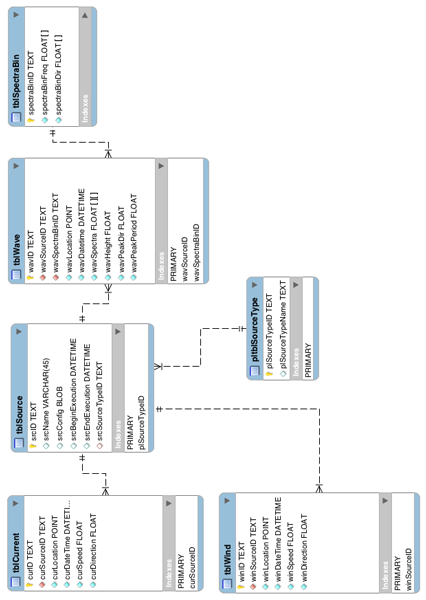
\includegraphics{../images/wave-database-20100720.png}
\caption{Preliminary Database Schematic}
\label{db-schematic}
\end{figure}

\subsection{Representing Data in Matlab}

For each type of data we process and analyze (wave, wind, current),
we commonly work with data distributed spatially over some
computational domain as well as temporally varying. For current and
wind data, we represent each component (either speed/direction or
U\_x/U\_y) with a three dimensional array (2 dimensions for space,
1 for time).

In order to work with wave spectra in a similar manner, we have to
collapse the spectral representation into something that can be
stored as a Matlab scalar. One option is to summarize the wave
spectra at each point into statistics such as significant wave
height, peak period, dominant direction, etc. However, information
important to our analysis is lost in the summary of spectra.

As an alternative, we utilize Matlab's object-oriented programming
capability. We define a class called waveSpectra, which stores the
one or two dimensional wave spectra at a single point. Methods
implemented for the class produce summary statistics or partition
the spectra into wave groups. An instance of the class can then be
represented in Matlab as a scalar and therefore placed into an
array of the same dimension and size as the wind or current data.

\subsection{Data Flow}


\subsection{Input Data Retrieval}

Before a CMS model run can be initiated, the appropriate input data must be collected, formatted, and specified in the appropriate configuration files.  In order to facilitate the use of CMS in a real-time context, the process of gathering data from online sources must be reliable and fully automated.  To accomplish this, we created a set of Python scripts to connect to remote data archives, parse the relevant data, and store to the PostgreSQL database (Table \ref{tab:inputHarvest}).  Python was chosen as a platform for this task due to the availability of extensive libraries that facilitate working with a wide variety of data formats.

\begin{table}[b!]
\caption{Python scripts for retrieval of input data to CMS.}
\begin{center}
{
\begin{tabular}{| llll |}
\hline
\textbf{Name} & \textbf{Description} & \textbf{Data Source} & \textbf{Destinations} \\
 \hline
getNDBCWind.py & retrieves wind data from & \footnotesize http://www.ndbc.noaa.gov/ & tblWind\\
& any specified NDBC buoy & & \\
 \hline
getNAM12Wind.py & retrieves gridded wind  & \footnotesize http://www.nco.ncep.noaa.gov & tblWind\\
& data from the WRF-NAM model & & \\
 \hline
getWW3Spectra.py & retrieves directional spectra  &\footnotesize ftp://polar.ncep.noaa.gov/ & tblWave,\\
&from WWIII output& & tblSpectraBin \\
 \hline
getHFRadar.py & retrieves gridded current data &\footnotesize http://www.sccoos.org & tblCurrent \\
& from HF Radar sources & & \\
\hline
\end{tabular}}
\end{center}
\label{tab:inputHarvest}
\end{table}

\newpage
\section{List of Acronyms}
\label{loacronyms} 
\begin{singlespace}
\begin{eqnarray*}
\mbox{} & = & \mbox{}\\
\mbox{ACE} & = & \mbox{Army Corps of Engineers}\\
\mbox{CMS} & = & \mbox{Coastal Modeling System}\\
\mbox{D3D} & = & \mbox{Delft 3D}\\
\mbox{GIS} & = & \mbox{Geographic Information System}\\
\mbox{NOAA} & = & \mbox{National Oceanic \& Atmospheric Administration}\\
\mbox{PG\&E} & = & \mbox{Pacific Gas and Electric}\\
\mbox{WEC} & = & \mbox{Wave Energy Converter}\\
\mbox{WRF-NAM} & = & \mbox{Weather and Research Forecast Model - North American Mesoscale}\\
\mbox{WWIII} & = & \mbox{Wave Watch III}\\
\end{eqnarray*}
\end{singlespace}


\bibliographystyle{plain}
\bibliography{/Users/colinsheppard/Documents/wave-git/wave/docs/WaveConnect}

\end{document}
